
前一节中,我们了解了杀毒器如何使用仅在运行时可用的数据,帮助开发人员以更高的精度执行健全性检查。我们还了解了如何制作自定义杀毒器。在本节中,我们将继续讨论利用运行时数据的思想,将这些信息用于另一个方面——编译器优化。

PGO是一种技术,它使用在运行时收集的统计信息,来支持更积极的编译器优化(相关文件已经收集了足够的运行时数据)。为了了解这样的数据是如何增强优化的,假设我们有以下C代码:

\begin{lstlisting}[style=styleCXX]
void foo(int N) {
	if (N > 100)
		bar();
	else
		zoo();
}
\end{lstlisting}

这段代码中,我们有三个函数:\texttt{foo}、\texttt{bar}和\texttt{zoo}。第一个函数有条件地调用后两个函数。

当我们尝试优化这段代码时,优化器通常会尝试将函数内联扩展到调用函数中。这种情况下,\texttt{bar}或\texttt{zoo}可能会内联到\texttt{foo}中。但是,如果\texttt{bar}或\texttt{zoo}有一个较大的函数体,内联两者可能会使最终二进制文件的体积膨胀。理想情况下,如果只能内联执行最频繁的那一个,那就太好了。遗憾的是,从统计的角度来看,我们不知道哪个函数的执行频率最高,因为\texttt{foo}函数根据一个(非常量)变量有条件地使用它们中的一个。

使用PGO,我们可以在运行时收集\texttt{bar}和\texttt{zoo}的执行频率,并使用这些数据再次编译(和优化)相同的代码。下图展示了这一理念的高层概述:

\hspace*{\fill} \\ %插入空行
\begin{center}
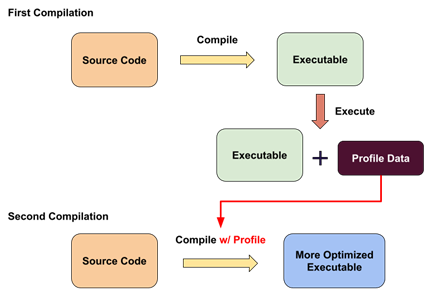
\includegraphics[width=0.8\textwidth]{content/3/chapter12/images/5.png}\\
图12.5 - PGO工作流
\end{center}

这里,第一个编译阶段通常编译和优化代码。在执行编译后的程序(任意次数)之后,能够收集到足够的运行数据文件。在第二个编译阶段,我们不仅像以前那样优化了代码,而且还将收集到的数据集成到优化中,以使它们更积极地发挥作用。

PGO主要有两种方法来收集运行时分析数据:插入\textbf{检测}代码或利用\textbf{采样}数据。


\subsubsubsection{12.3.1\hspace{0.2cm}基于检测的PGO}

基于检测的PGO在第一个编译阶段将检测代码插入到目标程序中。这段代码测量我们感兴趣的程序构造的执行频率——例如,基本块和函数——并将结果写入文件。这与杀毒器的工作原理类似。

基于检测的PGO通常生成精度更高的数据。这是因为编译器可以以一种为其他优化提供最大好处的方式插入检测代码。然而,就像杀毒器一样,基于检测的PGO改变了目标程序的执行流,不过这增加了性能回归的风险(对于从第一个编译阶段生成的二进制文件)。

\subsubsubsection{12.3.2\hspace{0.2cm}基于采样的PGO}

基于采样的PGO使用外部工具收集分析数据。开发人员使用\texttt{perf}或\texttt{valgrind}等分析器来诊断性能问题。这些工具通常利用高级的系统特性,甚至硬件特性来收集程序的运行时行为,例如:\texttt{perf}可以让您了解分支预测和缓存缺失。

因为我们正在利用来自其他工具的数据,所以不需要修改原始代码来收集概要文件。因此,基于采样的PGO通常具有极低的运行时开销(通常小于1\%)。此外,我们不需要为了分析目的而重新编译代码。然而,以这种方式生成的分析数据通常不那么精确。第二个编译阶段中,将分析数据映射回原始代码也更加困难。

本节的其余部分,我们将重点关注基于检测的PGO。我们将学习如何利用它与LLVM IR。然而,LLVM中的这两种PGO策略共享许多公共的工具,因此代码是可移植的。下面是我们将要讨论的内容:

\begin{itemize}
\item 使用分析数据
%\item 理解检测级别
\item 了解访问分析数据的API
\end{itemize}

第一个主题将向我们展示如何使用Clang创建和使用基于检测的PGO数据文件,以及一些可以帮助我们检查和修改概要数据文件的工具。第二个主题将提供更多关于如何使用LLVM API访问分析数据的详细信息。如果想创建自己的PGO Pass,这是很有用的。

\hspace*{\fill} \\ %插入空行
\noindent
\textbf{使用分析数据}

本节中,我们将了解如何使用生成、检查甚至修改基于工具的分析数据。让我们从下面的例子开始:

\begin{lstlisting}[style=styleCXX]
__attribute__((noinline))
void foo(int x) {
	if (get_random() > 5)
	printf("Hello %d\n", x * 3);
}
int main(int argc, char **argv) {
	for (int i = 0; i < argc + 10; ++i) {
		foo(i);
	}
	return 0;
}
\end{lstlisting}

上面的代码中,\texttt{get\_random}是一个函数,生成一个从1到10的均匀分布的随机数。换句话说,\texttt{foo}函数中突if语句应该有50\%的几率被执行。除了\texttt{foo}函数之外,\texttt{main}中的\texttt{for}循环的迭代计数取决于命令行参数的数量。

现在,让我们尝试使用基于检测的PGO构建这段代码。以下是步骤:

\begin{enumerate}
\item 第一件事是为PGO分析生成一个可执行文件。命令如下:

\begin{tcblisting}{commandshell={}}
$ clang -O1 -fprofile-generate=pgo_prof.dir pgo.cpp -o pgo
\end{tcblisting}

\texttt{-fprofile-generate}选项支持基于检测的PGO,我们在此标志之后添加的路径是存储分析数据的目录。

\item 接下来,必须使用三个命令行参数运行\texttt{pgo}:

\begin{tcblisting}{commandshell={}}
$ ./pgo `seq 1 3`
Hello 0
Hello 6
…
Hello 36
Hello 39
$
\end{tcblisting}

每个人可能会得到一个完全不同的输出,因为只有50\%的机会打印字符串。

在这之后,\texttt{pgo\_prof.dir}文件夹应该包含\texttt{default\_<hash>\_<n>.profraw}文件,如下所示:

\begin{tcblisting}{commandshell={}}
$ ls pgo_prof.dir 
default_10799426541722168222_0.profraw
\end{tcblisting}

文件名中的哈希值是基于代码计算的哈希值。

\item 不能直接使用\texttt{*.profraw}文件用于第二个编译阶段。相反,必须使用\texttt{llvm-profdata}工具将其转换为另一种二进制形式。命令如下:

\begin{tcblisting}{commandshell={}}
$ llvm-profdata merge pgo_prof.dir/ -o pgo_prof.profdata
\end{tcblisting}

\texttt{llvm-profdata}是一个强大的工具,用于检查、转换和合并分析数据文件,我们将在后面更详细地讨论它。上面的命令中,我们正在合并和转换\texttt{pgo\_prof.dir}下的所有数据文件,到单个\texttt{*.profdata}文件中。

\item 最后,我们可以使用合并的文件进行第二阶段的编译。命令如下:

\begin{tcblisting}{commandshell={}}
$ clang -O1 -fprofile-use=pgo_prof.profdata pgo.cpp \
        -emit-llvm -S -o pgo.after.ll
\end{tcblisting}

\end{enumerate}

这里,\texttt{-fprofile-use}选项告诉\texttt{clang}使用存储在\texttt{pgo\_prof.profdata}中的分析数据来优化代码。在完成这个优化之后,我们再来看看LLVM IR代码。

打开\texttt{pgo.after.ll},并找到到\texttt{foo}函数。下面是\texttt{foo}的简化版本:

\begin{lstlisting}[style=styleCXX]
define void @foo(i32 %x) !prof !71 {
entry:
	%call = call i32 @get_random()
	%cmp = icmp sgt i32 %call, 5
	br i1 %cmp, label %if.then, label %if.end, !prof !72
	
if.then:
	%mul = mul nsw i32 %x, 3
	…
}
\end{lstlisting}

在之前的LLVM IR代码中,有两个地方与原来的IR不同,紧跟在函数头文件和分支指令之后的\texttt{!prof}标记,它对应于我们前面看到的\texttt{if(get\_random() > 5)}。

在LLVM IR中,我们可以将\textbf{元数据}附加到不同的IR单元以提供补充信息。元数据将以一个以感叹号('!')开头的标签出现在文本LLVM IR中。前面代码中的\texttt{!prof}、\texttt{!71}和\texttt{!72}是表示我们收集的分析数据的元数据标记。更具体地说,如果我们有与IR单元相关联的分析数据,总是以\texttt{!prof}开头,然后是另一个元数据标记包含所需值。这些元数据值放在IR文件的最底部。如果在那里查找,会看到\texttt{!71}和\texttt{!72}的内容。代码如下:

\begin{tcblisting}{commandshell={}}
!71 = !{!"function_entry_count", i64 110}
!72 = !{!"branch_weights", i32 57, i32 54}
\end{tcblisting}

这两个元数据是包含两个和三个元素的元组。\texttt{!71},正如它的第一个元素所表示的,表示\texttt{foo}函数被调用的次数(在本例中,调用了110次)。

\texttt{!72}表示\texttt{if(get\_random() > 5)}语句中每个分支执行的次数。本例中,真分支走了57次,假分支走了54次。之所以会得到这样的数字,是因为我们使用均匀分布生成随机数(也就是说,每个分支有~50\%的概率)。

本节的第二部分中,我们将了解如何访问这些值,以便开发更积极的编译器优化。但在这样做之前,让我们更深入地了解我们刚刚收集的分析数据文件。

我们刚才使用的\texttt{llvm-profdata}工具,不仅可以帮助我们转换分析数据的格式,而且还可以为我们提供其内容的快速预览。下面的命令可以打印出\texttt{pgo\_prof.profdata}的内容,包括从每个函数中收集的分析值:

\begin{tcblisting}{commandshell={}}
$ llvm-profdata show –-all-functions –-counts pgo_prof.profdata
…
  foo:
    Hash: 0x0ae15a44542b0f02
    Counters: 2
    Block counts: [54, 57]
\end{tcblisting}

\begin{tcblisting}{commandshell={}}
  main:
    Hash: 0x0209aa3e1d398548
    Counters: 2
    Block counts: [110, 1]
…
Instrumentation level: IR entry_first = 0
Functions shown: 9
Total functions: 9
Maximum function count: …
Maximum internal block count: …
\end{tcblisting}

这里,我们可以看到每个函数的分析数据条目。每个条目都有一个数字列表,表示所有封闭的基本块的执行频率。

或者,可以先将相同的分析数据文件转换为文本文件,再来检查它。命令如下:

\begin{tcblisting}{commandshell={}}
$ llvm-profdata merge –-text pgo_prof.profdata -o pgo_prof.
proftext
$ cat pgo_prof.proftext
# IR level Instrumentation Flag
:ir
…
foo
# Func Hash:
784007059655560962
# Num Counters:
2
# Counter Values:
54
57
…
\end{tcblisting}

\texttt{*.proftext}文件是一种可读的文本格式,所有的分析数据都简单地放在相应行中。

这种文本表示实际上可以转换回\texttt{*.profdata}格式使用类似的命令:

\begin{tcblisting}{commandshell={}}
$ llvm-profdata merge –-binary pgo_prof.proftext -o pgo_prof.profdata
\end{tcblisting}

因此,\texttt{*.proftext}对于手动编辑分析数据比较友好。

在深入研究PGO的API之前,我们还需要了解一个概念:检测级别。

\hspace*{\fill} \\ %插入空行
\noindent
\textbf{检测级别}

到目前为止,我们已经了解到基于检测的PGO可以插入检测代码来收集运行时的分析数据,插入检测代码的位置,及其粒度也很重要。这个属性在基于工具的PGO中称为\textbf{检测级别}。LLVM目前支持三种不同的检测级别。以下是对它们的描述:

\begin{itemize}
\item \textbf{IR}: 检测代码是基于LLVM IR插入的,例如:收集已获取分支数量的代码直接插入到分支指令之前,\texttt{-fprofile-generate}命令行选项将用这个检测级别生成分析数据。假设我们有以下C代码:

\begin{lstlisting}[style=styleCXX]
void foo(int x) {
	if (x > 10)
		puts("hello");
	else
		puts("world");
}
\end{lstlisting}

对应的IR——不启用基于检测的PGO——如下所示:

\begin{lstlisting}[style=styleCXX]
define void @foo(i32 %0) {
	…
	%4 = icmp sgt i32 %3, 10
	br i1 %4, label %5, label %7
	
5:
	%6 = call i32 @puts(…"hello"…)
	br label %9
7:
	%8 = call i32 @puts(…"world"…)
	br label %9
	
9:
	ret void
}
\end{lstlisting}

这里有一个基本块的分支:\%5或\%7。现在,让我们使用下面的命令来生成基于检测的PGO的IR:

\begin{tcblisting}{commandshell={}}
$ clang -fprofile-generate -emit-llvm -S input.c
\end{tcblisting}

这与我们在使用分析数据部分中,用于第一个PGO编译阶段的命令相同,只不过我们生成的是LLVM IR,而不是可执行文件。得到的IR如下所示:

\begin{lstlisting}[style=styleCXX]
define void @foo(i32 %0) {
	…
	%4 = icmp sgt i32 %3, 10
	br i1 %4, label %5, label %9
5:
	%6 = load i64, i64* … @__profc_foo.0, align 8
	%7 = add i64 %6, 1
	store i64 %7, i64* … @__profc_foo.0, align 8
	%8 = call i32 @puts(…"hello"…)
	br label %13
9:
	%10 = load i64, i64* … @__profc_foo.1, align 8
	%11 = add i64 %10, 1
	store i64 %11, i64* … @__profc_foo.1, align 8
	%12 = call i32 @puts(…"world"…)
	br label %13
	
13:
	ret void
}
\end{lstlisting}

上面的IR中,两个分支中的基本块都有新的代码。更具体地说,两者都增加全局变量的值—\texttt{—@\_\_profc\_foo.0}或\texttt{@\_\_profc\_foo.1}。这两个变量中的值最终将导出为分支的分析数据,从而表示每个分支的使用次数。

这个检测级别提供了相当好的精度,但会受到编译器更改的影响。更具体地说,如果Clang改变了它生成LLVM IR的方式,那么插入检测代码的位置也会不同。这意味着对于相同的输入代码,使用旧版本的LLVM生成的分析数据可能与使用新版本的LLVM生成的分析数据不兼容。

\item \textbf{AST}: 检测代码是基于AST插入的,例如:收集已获取分支数量的代码可以作为\texttt{IfStmt}(一个AST节点)中的一个新的texttt{Stmt} AST节点插入。使用此方法,检测代码几乎不受编译器更改的影响,我们可以在不同编译器版本之间拥有更稳定的分析数据格式。这个检测级的缺点是它的精度低于IR检测级。

第一次编译使用\texttt{clang}时,只需使用\texttt{-fprofile-instrgenerate}命令行选项代替\texttt{-fpro\\file-generate},就可以采用这种检测级别。但是,在第二次编译时不需要更改命令。

\item \textbf{上下文敏感}: 使用分析数据部分中,我们了解到可以收集关于分支执行次数的信息。然而,在IR检测级别上,几乎不可能知道哪个是使用最多的分支。换句话说,传统的IR检测级别失去了调用的上下文。上下文敏感的检测级别,试图通过在函数内联后,再次收集概要文件来解决这个问题,从而获取更高精度的数据。

然而,在Clang中使用这个特性有点麻烦——我们需要编译相同的代码三次,而不是两次。以下是使用上下文敏感的PGO步骤:

\begin{tcblisting}{commandshell={}}
$ clang -fprofile-generate=first_prof foo.c -o foo_exe
$ ./foo_exe …
$ llvm-profdata merge first_prof -o first_prof.profdata
\end{tcblisting}

首先,使用我们在“使用分析数据”一节中学到的内容,生成一些普通的(IR检测级)分析数据:

\begin{tcblisting}{commandshell={}}
$ clang -fprofile-use=first_prof.profdata \
        -fcs-profile-generate=second_prof foo.c -o foo_exe2
$ ./foo_exe2
$ llvm-profdata merge first_prof.profdata second_prof \
          -o combined_prof.profdata
\end{tcblisting}

然后,使用两个PGO命令行选项运行\texttt{clang},\texttt{-fprofile-use}和\texttt{-fc-profile-generate},分别带有上一步的配置文件路径和预期的输出路径。当使用\texttt{llvm-profdata}来做后处理时,我们合并了所有的数据文件:

\begin{tcblisting}{commandshell={}}
$ clang -fprofile-use=combined_prof.profdata \
        foo.c -o optimized_foo
\end{tcblisting}

最后,将组合的分析文件输入到Clang中,这样Clang就可以使用上下文敏感的分析数据来更准确地描述程序的运行时行为。

\end{itemize}

注意,不同的检测级别只会影响数据的准确性,它们不会影响我们如何检索这些数据,这将在下一节中进行讨论。

本节的最后一部分,我们将了解如何通过LLVM提供的API访问LLVM Pass中的分析数据。

\hspace*{\fill} \\ %插入空行
\noindent
\textbf{了解访问分析数据的API}

前一节中,我们学习了如何使用Clang运行基于检测的PGO,并使用\texttt{llvm-profdata}查看分析数据文件。本节中,我们将了解如何在LLVM Pass中访问数据,以助于开发自己的PGO。

深入开发细节之前,让我们了解一下如何将这些分析数据文件使用到\texttt{opt}中,因为使用它更容易测试单个LLVM Pass。下面是一个示例命令:

\begin{tcblisting}{commandshell={}}
$ opt -pgo-test-profile-file=pgo_prof.profdata \
      --passes="pgo-instr-use,my-pass…" pgo.ll …
\end{tcblisting}

上面的命令中有两个关键:

\begin{itemize}
\item 使用\texttt{-pgo-test-profile-file}指定要写入的分析数据文件。

\item "pgo-in-use"字符串表示\texttt{PGOInstrumentaitonUse} Pass,它读取(基于检测的)数据文件,并在LLVM IR上注释数据。但是,即使在预定义的优化级别(即O0 ~ O3、Os和Oz)中,也不会默认运行。如果Pass不在pass流水的前部,我们就无法访问任何分析数据。因此,我们需要显式地将其添加到优化流水中。前面的示例命令演示了如何在管道中运行自定义LLVM Pass(\texttt{my-pass})之前运行。如果想在任何预定义的优化流水(例如O1)之前运行,必须指定\texttt{-\,-passes="pgo-inst -use,default<O1>"}命令行选项。
\end{itemize}

现在,在将分析数据读入\texttt{opt}之后会发生什么?由第二个编译阶段(\texttt{pgo.after.ll})生成的LLVM IR文件,会为我们提供了这个问题的答案。

在\texttt{pgo.after.ll}中,我们看到一些分支使用元数据装饰,这些元数据获取它们的次数。类似的元数据出现在函数中,表示这些函数调用的总次数。

更一般地说,LLVM通过元数据直接将数据(从文件中读取)与相关的IR结构结合在一起。这种策略的最大优点是,不需要在整个优化过程中携带原始分析数据——IR本身包含了这个分析信息。

现在的问题是,我们如何访问附加到IR的元数据?LLVM的元数据可以附加到多种IR单元上。让我们先来看看最常见的一个:访问附加到指令的元数据。下面的代码向我们展示了如何读取分析元数据——\texttt{!prof !71},它附加到一个分支指令上:

\begin{lstlisting}[style=styleCXX]
// `BB` has the type of `BasicBlock&`
Instruction *BranchInst = BB.getTerminator();
MDNode *BrWeightMD = BranchInst->getMetadata(LLVMContext::MD_
prof);
\end{lstlisting}

上面的代码段中,我们使用\texttt{BasicBlock::getTerminator}来获取基本块中的最后一条指令,这在大多数情况下是一条分支指令。然后,我们尝试使用\texttt{MD\_prof}元数据检索分析元数据。\texttt{BrWeightMD}是我们正在寻找的结果。
 
\texttt{BrWeightMD}的类型\texttt{MDNode}表示单个元数据节点。不同的\texttt{MDNode}实例可以组合在一起。一个\texttt{MDNode}实例可以使用其他\texttt{MDNode}实例作为它的操作数——类似于在第10章中的实例。复合\texttt{MDNode}可以表达更复杂的概念。

在本例中,\texttt{BrWeightMD}中的每个操作数表示获取每个分支的次数。下面是访问代码:

\begin{lstlisting}[style=styleCXX]
if (BrWeightMD->getNumOperands() > 2) {
	// Taken counts for true branch
	MDNode *TrueBranchMD = BrWeightMD->getOperand(1);
	// Taken counts for false branch
	MDNode *FalseBranchMD = BrWeightMD->getOperand(2);
}
\end{lstlisting}

计数也表示为\texttt{MDNode}。

\begin{tcolorbox}[colback=blue!5!white,colframe=blue!75!black, fonttitle=\bfseries,title=两个分支的操作数索引]	
\hspace*{0.7cm}注意,两个分支的数据都从索引1开始的操作数上,而不是索引0。
\end{tcolorbox}

如果希望将这些分支\texttt{MDNode}实例转换为常量,可以利用\texttt{mdconst}名称空间提供的一个小工具。下面是一个例子:

\begin{lstlisting}[style=styleCXX]
if (BrWeightMD->getNumOperands() > 2) {
	// Taken counts for true branch
	MDNode *TrueBranchMD = BrWeightMD->getOperand(1);
	ConstantInt *NumTrueBrTaken
	  = mdconst::dyn_extract<ConstantInt>(TrueBranchMD);
	…
}
\end{lstlisting}

前面的代码解包装了一个\texttt{MDNode}实例并提取了底层的\texttt{ConstantInt}实例。

对于\texttt{Function},可以用更简单的方法得到调用的次数:

\begin{lstlisting}[style=styleCXX]
// `F` has the type of `Function&`
Function::ProfileCount EntryCount = F.getEntryCount();
uint64_t EntryCountVal = EntryCount.getCount();
\end{lstlisting}

\texttt{Function}使用一种略有不同的方式来表示其调用的频率。但是检索数值分析值仍然非常容易,如上的代码所示。

值得注意的是,虽然这里只关注基于检测的PGO,但对于基于采样的PGO, LLVM也使用相同的编程接口来公开其数据。换句话说,即使正在使用从使用不同的\texttt{opt}命令的采样工具收集的分析数据,分析数据也将标注在IR单元上,仍然可以使用上述方法访问。实际上,在本节的其余部分中,我们将介绍的工具和API,大多与分析数据源无关。

目前为止,我们一直在处理从分析数据中检索到的实际值。然而,在开发编译器优化或程序分析算法方面,这些低层值不能帮助我们走得太远——通常,我们更感兴趣的是高级概念,如“最频繁执行的函数”或“最少执行的分支”。为了满足这些需求,LLVM在分析数据的基础上构建了几个分析,以提供这种高级的结构化信息。

下一节中,我们将介绍其中的一些分析,以及在LLVM Pass中的用法。

\subsubsubsection{12.3.3\hspace{0.2cm}使用性能数据进行分析}

在本节中,我们将学习三个分析类,它们可以帮助我们推断基本块和函数在运行时的执行频率。具体如下:

\begin{itemize}
\ttfamily
\item BranchProbabilityInfo
\item BlockFrequencyInfo
\item ProfileSummaryInfo
\end{itemize}

这个列表是按照它们在IR中的分析范围排序的——从本地到全局。让我们从前两个开始。

\hspace*{\fill} \\ %插入空行
\noindent
\textbf{使用BranchProbabilityInfo和BlockFrequencyInfo}

在前一节中,我们了解了如何访问附加到每个分支指令的分析元数据——\textbf{分支权重}。LLVM中的分析框架通过\texttt{BranchProbabilityInfo}类提供了一种更简单的方法来访问这些值。下面是一些示例代码,展示了如何在(函数)Pass中使用它:

\begin{lstlisting}[style=styleCXX]
#include "llvm/Analysis/BranchProbabilityInfo.h"
PreservedAnalyses run(Function &F, FunctionAnalysisManager
&FAM) {
	BranchProbabilityInfo &BPI
	  = FAM.getResult<BranchProbabilityAnalysis>(F);
	BasicBlock *Entry = F.getEntryBlock();
	BranchProbability BP = BPI.getEdgeProbability(Entry, 0);
	…
}
\end{lstlisting}

前面的代码检索了\texttt{BranchProbabilityInfo}的实例,是\texttt{BranchProbabilityAnalysis}的结果,并试图从入口块获取到其第一个后续块的权重。

返回值是一个\texttt{BranchProbability}实例,它以百分比的形式给出了分支的概率。可以使用\texttt{BranchProbability::getNumerator}检索值(“分母”默认为100)。\texttt{BranchProbability}类还提供了一些方便的实用方法,用于在两个分支概率之间执行算术,或按特定因子缩放概率。尽管使用\texttt{BranchProbabilityInfo}可以很容易地知道哪个分支更有可能走到,但是没有额外的数据,我们不能在整个函数中告诉执行分支的概率,例如:假设我们有以下CFG:

\hspace*{\fill} \\ %插入空行
\begin{center}
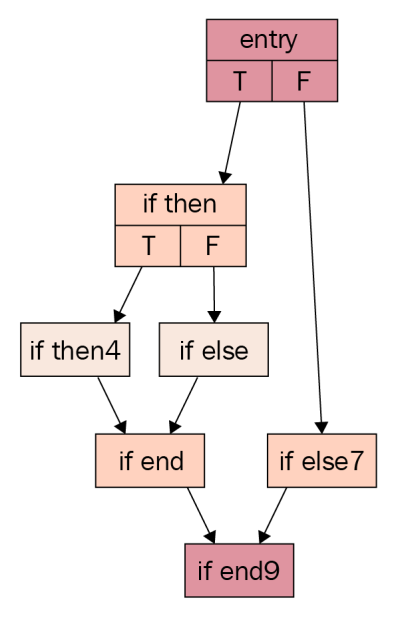
\includegraphics[width=0.3\textwidth]{content/3/chapter12/images/6.png}\\
图12.6 - CFG嵌套分支
\end{center}

对于上图,我们有以下基本块的分析计数器值:

\begin{itemize}
\ttfamily
\item \textbf{if.then4}: 2
\item \textbf{if.else}: 10
\item \textbf{if.else7}: 20
\end{itemize}

如果我们只看分支权重元数据块\texttt{if.then4}和\texttt{if.else}——即\texttt{if.then}的真和假分支。然后,我们可能会产生一种错觉,\texttt{if.else}块有~83\%的几率。但事实是,只有~31\%的概率,因为控制流进入在进入\texttt{if.then}之前,\texttt{if.else7}的概率更高。在这种情况下,我们可以通过计算来得出正确的答案,但当CFG变得更大更复杂时,我们就很难自己做判断了。

\texttt{BlockFrequencyInfo}类提供了解决这个问题的捷径。它可以告诉我们每个基本块在其封闭函数的上下文中执行的频率。下面是它在Pass中的用法:

\begin{lstlisting}[style=styleCXX]
#include "llvm/Analysis/BlockFrequencyInfo.h"
PreservedAnalyses run(Function &F, FunctionAnalysisManager
&FAM) {
	BlockFrequencyInfo &BFI
	  = FAM.getResult<BlockFrequencyAnalysis>(F);
	for (BasicBlock *BB : F) {
		BlockFrequency BF = BFI.getBlockFreq(BB);
	}
	…
}
\end{lstlisting}

前面的代码检索了\texttt{BlockFrequencyInfo}实例,是\texttt{BlockFrequencyAnalysis}的结果,并尝试计算函数中每个基本块的块频率。

类似于\texttt{BranchProbability}类,\texttt{BlockFrequency}也提供了方法来计算其他\texttt{BlockFrequency}实例。但与\texttt{BranchProbability}不同,从\texttt{BlockFrequency}检索到的数值不是以百分比表示的。\texttt{BlockFrequency::getFrequency}返回一个整数,是相对于当前函数的入口块的频率。要获得基于百分比的频率,可以使用下面的代码:

\begin{lstlisting}[style=styleCXX]
// `BB` has the type of `BasicBlock*`
// `Entry` has the type of `BasicBlock*` and represents entry
// block
BlockFrequency BBFreq = BFI.getBlockFreq(BB),
               EntryFreq = BFI.getBlockFreq(Entry);
auto FreqInPercent
  = (BBFreq.getFrequency() / EntryFreq.getFrequency()) * 100;
\end{lstlisting}

\texttt{FreqInPercent}表示\texttt{BB}的阻塞频率,以百分比表示。

\texttt{BlockFrequencyInfo}在函数的上下文中计算特定基本块的频率——但是整个模块呢?如果在这种情况下引入调用图,是否可以将我们刚刚学过的块频率与调用函数的频率相乘,以得到全局范围内的执行频率?幸运的是,LLVM已经准备了一个有用的类来解决这个问题——\texttt{ProfileSummaryInfo}。

\hspace*{\fill} \\ %插入空行
\noindent
\textbf{使用ProfileSummaryInfo}

\texttt{ProfileSummaryInfo}类提供了一个模块中所有分析数据的全局视图。下面是一个在模块中检索实例的例子:

\begin{lstlisting}[style=styleCXX]
#include "llvm/Analysis/ProfileSummaryInfo.h"
PreservedAnalyses run(Module &M, ModuleAnalysisManager &MAM) {
	ProfileSummaryInfo &PSI = MAM.
	getResult<ProfileSummaryAnalysis>(M);
	…
}
\end{lstlisting}

\texttt{ProfileSummaryInfo}提供了各种各样的功能。让我们来看看它最有意思的三个方法:

\begin{itemize}
\item \texttt{isFunctionEntryCold/Hot(Function*)}: 这两种方法将\texttt{Function}的输入计数(有效地反映了函数被调用的次数)与同一模块中其他函数的输入计数进行比较,并告诉我们查询函数在这个指标中的排名是高还是低。

\item \texttt{isHot/ColdBlock(BasicBlock*, BlockFrequencyInfo\&)}: 这两个方法的工作方式与前面的项目一相似,但比较的是\texttt{BasicBlock}与模块中所有其他块的执行频率.

\item \texttt{isFunctionCold/HotInCallGraph(Function*,
BlockFrequencyInfo\&)}: 这两个方法结合了前面两个要点的方法,可以根据函数的入口计数,或其封闭基本块的执行频率来判断函数是“热”的,还是“冷”的。当一个函数有一个很低的输入计数(也就是说,它不经常被调用),但是包含一个具有极高的基本块执行频率的循环时,这是很有用的。在本例中,\texttt{isFunctionHotInCallGraph}方法可以给我们一个更准确的评估。

\end{itemize}

这些API还有变体,可以自定义“热”与“冷”的分界点。有关更多信息,请参阅API文档。

很长一段时间,编译器只能用静态视图分析和优化源代码。对于程序内部的动态因素——例如,有计数的分支——编译器只能做出一个近似值。PGO打开了格局,为编译器提供额外的信息,以查看目标程序的运行时行为,以便做出更明确和更积极的决策。本节中,我们了解了如何使用LLVM收集和使用运行时概要信息(PGO的关键)。我们了解了如何在LLVM中使用相关的工具来收集和生成这样的概要数据。我们还了解了我们用来访问数据的编程接口——以及在此基础上构建的一些高级分析——以帮助我们在LLVM Pass中进行开发。有了这些功能,LLVM开发人员就可以插入这些运行时信息,进一步提高现有优化过程的质量和精度。














